\documentclass[11pt, reqno]{article}    % use "amsart" instead of "article" for AMSLaTeX format
\usepackage{my_packages}
\usepackage{tikz_packages}
\usepackage{pgfplots}
\pgfplotsset{compat=1.14}
\usepackage[explicit]{titlesec}
\titleformat{\section}[runin]{\normalfont\bfseries}{}{0em}{#1\ \thesection}

\title{MAE 3134: Homework 7}
\author{Shankar Kulumani}
\date{Spring 2017}                          % Activate to display a given date or no date

\begin{document}
{\noindent\Large \textbf{MAE 3134: Homework 7}}

\noindent \textbf{Due date}: 13 April 2017, 0935 \\
\section{Problem}
For each of the systems identified below, copmute the magnitude and angle of the transfer function when evaluated at the specified points in the imaginary plane (s-plane).
You should use algebra to transform each function into a general complex number, then evaluate at each desired point. 
You must show your work for full credit.
The magnitude should be reported in decibels~(\si{\decibel}) and the angle in degrees.
\begin{enumerate}
    \item Accelerometer model:
    \begin{align*}
        G(s) = \frac{X(s)}{F(s)} = \frac{0.5}{s^2 + 2 s + 10}
    \end{align*}
    evaluated at the following points:
    \begin{enumerate}
        \item \( s = j 2\) 
        \item \( s = j 3.1623\)
        \item \( s = j 2.8284\)
    \end{enumerate}
    \item Low-pass filter:
    \begin{align*}
        G(s) = \frac{V_{out}(s)}{V_{in}(s)} = \frac{5}{s + 6}
    \end{align*}
    evaluated at the following points:
    \begin{enumerate}
        \item \( s = j 0.6\) 
        \item \( s = j 6\)
        \item \( s = j 60\)
    \end{enumerate}
    \item High-pass filter:
    \begin{align*}
        G(s) = \frac{V_{out}(s)}{V_{in}(s)} = \frac{s}{s + 35}
    \end{align*}
    evaluated at the following points:
    \begin{enumerate}
        \item \( s = j 2\) 
        \item \( s = j 35\)
        \item \( s = j 500\)
    \end{enumerate}
    \item Lead filter:
    \begin{align*}
        G(s) = \frac{V_{out}(s)}{V_{in}(s)} = \frac{0.21(s+2)}{s + 3.05}
    \end{align*}
    evaluated at the following points:
    \begin{enumerate}
        \item \( s = j 0.247\) 
        \item \( s = j 2.47\)
        \item \( s = j 24.7\)
    \end{enumerate}
\end{enumerate}

\clearpage

\noindent\textbf{You should produce HIGH quality Bode plots using the approximation tools learned in class. 
This means that you should use a ruler and write neatly and clearly.}

\section{Problem}
Using the tranfer function of the \textbf{accelerometer model} given in~Problem 1:
\begin{enumerate}
    \item Draw an asymptotic Bode plot on the graphs provided.
    \item Plot the true magnitude and phase of the specific points given previously.
    \item Sketch your estimate of the actual Bode plot.
\end{enumerate}

\begin{figure*}[htbp] 
    \centering 
    \begin{subfigure}[htbp]{\textwidth} 
    \begin{tikzpicture}[]
        \begin{semilogxaxis}[
            xmin=1e0, xmax=1e4,
            ymin=0, ymax=10,
            grid=both,
            grid style={line width=0.1pt, draw=gray!25},
            major grid style={line width=0.2pt, draw=gray!75},
            yticklabels={,,},
            xticklabels={,,},
            minor tick num=4,
            width=\textwidth,
            height=0.43\textheight
        ]
        \end{semilogxaxis}
    \end{tikzpicture}
    \vspace*{0.2cm}
    \end{subfigure}

    \begin{subfigure}[htbp]{\textwidth} 
    \begin{tikzpicture}[]
        \begin{semilogxaxis}[
            xmin=1e0, xmax=1e4,
            ymin=0, ymax=10,
            grid=both,
            grid style={line width=0.1pt, draw=gray!25},
            major grid style={line width=0.2pt, draw=gray!75},
            yticklabels={,,},
            xticklabels={,,},
            minor tick num=4,
            width=\textwidth,
            height=0.43\textheight
        ]
        \end{semilogxaxis}
    \end{tikzpicture}
    \end{subfigure}
\end{figure*}

\clearpage

\noindent\textbf{You should produce HIGH quality Bode plots using the approximation tools learned in class. 
This means that you should use a ruler and write neatly and clearly.}
\section{Problem}
Using the tranfer function of the \textbf{low-pass filter} given in~Problem 1:
\begin{enumerate}
    \item Draw an asymptotic Bode plot on the graphs provided.
    \item Plot the true magnitude and phase of the specific points given previously.
    \item Sketch your estimate of the actual Bode plot.
\end{enumerate}

\begin{figure*}[htbp] 
    \centering 
    \begin{subfigure}[htbp]{\textwidth} 
    \begin{tikzpicture}[]
        \begin{semilogxaxis}[
            xmin=1e0, xmax=1e4,
            ymin=0, ymax=10,
            grid=both,
            grid style={line width=0.1pt, draw=gray!25},
            major grid style={line width=0.2pt, draw=gray!75},
            yticklabels={,,},
            xticklabels={,,},
            minor tick num=4,
            width=\textwidth,
            height=0.43\textheight
        ]
        \end{semilogxaxis}
    \end{tikzpicture}
    \vspace*{0.2cm}
    \end{subfigure}

    \begin{subfigure}[htbp]{\textwidth} 
    \begin{tikzpicture}[]
        \begin{semilogxaxis}[
            xmin=1e0, xmax=1e4,
            ymin=0, ymax=10,
            grid=both,
            grid style={line width=0.1pt, draw=gray!25},
            major grid style={line width=0.2pt, draw=gray!75},
            yticklabels={,,},
            xticklabels={,,},
            minor tick num=4,
            width=\textwidth,
            height=0.43\textheight
        ]
        \end{semilogxaxis}
    \end{tikzpicture}
    \end{subfigure}
\end{figure*}

\clearpage

\noindent\textbf{You should produce HIGH quality Bode plots using the approximation tools learned in class. 
This means that you should use a ruler and write neatly and clearly.}
\section{Problem}
Using the tranfer function of the \textbf{high-pass filter} given in~Problem 1:
\begin{enumerate}
    \item Draw an asymptotic Bode plot on the graphs provided.
    \item Plot the true magnitude and phase of the specific points given previously.
    \item Sketch your estimate of the actual Bode plot.
\end{enumerate}

\begin{figure*}[htbp] 
    \centering 
    \begin{subfigure}[htbp]{\textwidth} 
    \begin{tikzpicture}[]
        \begin{semilogxaxis}[
            xmin=1e0, xmax=1e4,
            ymin=0, ymax=10,
            grid=both,
            grid style={line width=0.1pt, draw=gray!25},
            major grid style={line width=0.2pt, draw=gray!75},
            yticklabels={,,},
            xticklabels={,,},
            minor tick num=4,
            width=\textwidth,
            height=0.43\textheight
        ]
        \end{semilogxaxis}
    \end{tikzpicture}
    \vspace*{0.2cm}
    \end{subfigure}

    \begin{subfigure}[htbp]{\textwidth} 
    \begin{tikzpicture}[]
        \begin{semilogxaxis}[
            xmin=1e0, xmax=1e4,
            ymin=0, ymax=10,
            grid=both,
            grid style={line width=0.1pt, draw=gray!25},
            major grid style={line width=0.2pt, draw=gray!75},
            yticklabels={,,},
            xticklabels={,,},
            minor tick num=4,
            width=\textwidth,
            height=0.43\textheight
        ]
        \end{semilogxaxis}
    \end{tikzpicture}
    \end{subfigure}
\end{figure*}

\clearpage

\noindent\textbf{You should produce HIGH quality Bode plots using the approximation tools learned in class. 
This means that you should use a ruler and write neatly and clearly.}
\section{Problem} 
Using the tranfer function of the \textbf{lead filter} given in~Problem 1:
\begin{enumerate}
    \item Draw an asymptotic Bode plot on the graphs provided.
    \item Plot the true magnitude and phase of the specific points given previously.
    \item Sketch your estimate of the actual Bode plot.
\end{enumerate}

\begin{figure*}[htbp] 
    \centering 
    \begin{subfigure}[htbp]{\textwidth} 
    \begin{tikzpicture}[]
        \begin{semilogxaxis}[
            xmin=1e0, xmax=1e4,
            ymin=0, ymax=10,
            grid=both,
            grid style={line width=0.1pt, draw=gray!25},
            major grid style={line width=0.2pt, draw=gray!75},
            yticklabels={,,},
            xticklabels={,,},
            minor tick num=4,
            width=\textwidth,
            height=0.43\textheight
        ]
        \end{semilogxaxis}
    \end{tikzpicture}
    \vspace*{0.2cm}
    \end{subfigure}

    \begin{subfigure}[htbp]{\textwidth} 
    \begin{tikzpicture}[]
        \begin{semilogxaxis}[
            xmin=1e0, xmax=1e4,
            ymin=0, ymax=10,
            grid=both,
            grid style={line width=0.1pt, draw=gray!25},
            major grid style={line width=0.2pt, draw=gray!75},
            yticklabels={,,},
            xticklabels={,,},
            minor tick num=4,
            width=\textwidth,
            height=0.43\textheight
        ]
        \end{semilogxaxis}
    \end{tikzpicture}
    \end{subfigure}
\end{figure*}

\section{Problem} Answer the following questions:
\begin{enumerate}
    \item The model for a typical spring-mass-damper accelerometer is:
    \begin{align*}
         G(s) = \frac{X(s)}{F(s)} = \frac{0.5}{s^2 + 2 s + 10} .
    \end{align*}
    If the input to this system is
    \begin{align*}
        f(t) = 17.333 \sin 2 t ,
    \end{align*}
    what is the steady-state output of the system?
    \item We can model a low-pass filter as
    \begin{align*}
        G(s) = \frac{V_{out}(s)}{V_{in}(s)} = \frac{5}{s + 6} .
    \end{align*}
    For the following inputs, determine the steady-state output of the system:
    \begin{enumerate}
        \item \( v(t) = 10 \sin 0.6 t\)
        \item \( v(t) = 10 \sin 60 t\)
    \end{enumerate}
    Explain in your own words why this transfer funciton is called a ``low-pass filter''.
    \item Now let's look at the high-pass filter modeled as
    \begin{align*}
        G(s) = \frac{V_{out}(s)}{V_{in}(s)} = \frac{s}{s + 35} .
    \end{align*}
    Determine the steady-state output corresponding to these inputs:
    \begin{enumerate}
        \item \( v(t) = 10 \sin 2 t\)
        \item \( v(t) = 10 \sin 500 t\)
    \end{enumerate}
    Explain in your own words why this transfer function is called a ``high-pass filter''.
\end{enumerate}


\end{document}  
